% =====================================================================
%  JURNAL RESTI 2026 -- LaTeX template (Overleaf)
%  Reproduces TemplateRESTI2026.docx: A4, 25 mm margins, two columns
%  (4 mm gap), Times 10 pt, 6 pt paragraph spacing, IEEE references.
%  Compile with pdfLaTeX + BibTeX (Overleaf default). Files needed:
%    main.tex, references.bib, figures/logo_iaii.png
% =====================================================================
\documentclass[10pt,a4paper,twocolumn]{article}

% ---------- Page geometry (template: A4, 25 mm all sides) ------------
\usepackage[a4paper,top=25mm,bottom=25mm,left=25mm,right=25mm,
            columnsep=4mm,headheight=12pt,headsep=5mm,footskip=9mm]{geometry}

% ---------- Fonts: Times New Roman look-alike -------------------------
\usepackage[T1]{fontenc}
\usepackage[utf8]{inputenc}
\usepackage{newtxtext,newtxmath}
\usepackage{microtype}
\usepackage{xcolor}

% ---------- Packages ---------------------------------------------------
\usepackage{amsmath}
\usepackage{graphicx}
\usepackage{booktabs}      % tables without vertical lines (template rule)
\usepackage{array}
\newcolumntype{C}[1]{>{\centering\arraybackslash}p{#1}} % centred fixed-width column
\usepackage{caption}
\usepackage{titlesec}
\usepackage{fancyhdr}
\usepackage{ragged2e}      % \justifying inside the abstract block
\usepackage{cite}          % numeric citations: [1], [2], [4]--[6]
\usepackage[hidelinks]{hyperref}
\usepackage{url}

% ---------- Paragraphs: justified, no indent, 6 pt spacing -----------
\setlength{\parindent}{0pt}
\setlength{\parskip}{6pt plus 1pt minus 1pt}
\sloppy

% ---------- Section headings -------------------------------------------
% Heading 1: bold, 10 pt;  Heading 2: italic, 10 pt
\renewcommand{\thesection}{\arabic{section}}
\titleformat{\section}{\normalfont\normalsize\bfseries}{\thesection.}{0.5em}{}
\titleformat{\subsection}{\normalfont\normalsize\itshape}{\thesubsection}{0.5em}{}
\titlespacing*{\section}{0pt}{12pt}{6pt}
\titlespacing*{\subsection}{0pt}{10pt}{3pt}

% ---------- Captions: 8 pt, centred; table caption on top ------------
\captionsetup{font=footnotesize,labelsep=period,justification=centering,
              singlelinecheck=true,skip=4pt}
\captionsetup[table]{position=top}
\captionsetup[figure]{position=bottom}

% ---------- Equation spacing -----------------------------------------
\setlength{\abovedisplayskip}{6pt}
\setlength{\belowdisplayskip}{6pt}

% ---------- Header / footer (header from page 2, number bottom right) -
\newcommand{\shortauthors}{Wadagraprana \textit{et al.}}
\newcommand{\volinfo}{Jurnal RESTI Vol.\ x No.\ x (2026)}
\pagestyle{fancy}
\fancyhf{}
\fancyhead[L]{\footnotesize \shortauthors}
\fancyhead[R]{\footnotesize \volinfo}
\fancyfoot[R]{\footnotesize\thepage}
\renewcommand{\headrulewidth}{0.4pt}
\renewcommand{\footrulewidth}{0pt}
\fancypagestyle{firstpage}{%
  \fancyhf{}
  \fancyfoot[R]{\footnotesize\thepage}
  \renewcommand{\headrulewidth}{0pt}}

% ---------- References: 8 pt, IEEE ------------------------------------
\renewcommand{\refname}{References}

% =====================================================================
\begin{document}

% ---------------------------------------------------------------------
%  FIRST-PAGE BLOCK (single column, spans both columns)
% ---------------------------------------------------------------------
\twocolumn[{%
\centering
{\footnotesize Available online at website: \url{https://jurnal.iaii.or.id/index.php/RESTI}\par}
\vspace{0pt}
\par\vspace{0pt}\noindent\rule{\textwidth}{0.6pt}\par\vspace{0pt}

% Journal banner
\noindent
\begin{tabular}{@{}m{18mm}@{\hspace{3mm}}m{136mm}@{}}
  
\includegraphics[height=15mm]{figures/logo_iaii.png} &
  \begin{minipage}[c]{\linewidth}
    \centering

    {\fontsize{18pt}{18pt}\bfseries
      \textcolor[RGB]{0,102,166}{JURNAL RESTI}\par}

    \vspace{1pt}

    {\fontsize{14pt}{14pt}\selectfont\bfseries\bfseries
      \textcolor[RGB]{0,155,75}{(Rekayasa Sistem dan Teknologi Informasi)}\par}

    \vspace{2pt}

    {\footnotesize
      \raggedright
      Vol.\ x No.\ x (2026) xx -- xx
      \hfill e-ISSN: 2580-0760\par}
  \end{minipage}
\end{tabular}

\par\vspace{2pt}
\noindent\rule{\textwidth}{0.6pt}
\par\vspace{10pt}


% Title: Times 15 pt, not bold, max 12 words, only first letter capitalised
{\fontsize{15}{18}\selectfont
 Big Five Personality Prediction Using Swin Transformer and Multimodal Facial Features\par}
\vspace{8pt}

% Authors: 10 pt; * marks the corresponding author
{\normalsize
 Lalu Aldo Wadagraprana\textsuperscript{1},
 Candra Ayu Dewi\textsuperscript{1},
 Mohammad Nasyikh Al-Qusyairy\textsuperscript{1},
 David Ochieng' Agit\textsuperscript{1},
 Sarwosri Sarwosri\textsuperscript{1*}\par}
\vspace{4pt}

% Affiliations and e-mails: 9 pt
{\fontsize{9}{11}\selectfont
 \textsuperscript{1}Departemen Teknik Informatika, Fakultas Teknologi Elektro dan
 Informatika Cerdas, Institut Teknologi Sepuluh Nopember, Surabaya, Indonesia\par
 \vspace{2pt}
 \texttt{6025261052@student.its.ac.id}, \texttt{6025261001@student.its.ac.id}, \texttt{6025261008@student.its.ac.id},
 \texttt{6025261040@student.its.ac.id},
 \texttt{sarwosri@its.ac.id}\par
 \vspace{2pt}
 *Email corresponding author: \texttt{sarwosri@its.ac.id}\par}
\vspace{8pt}

% Abstract: heading bold 10 pt; text 9 pt italic, one paragraph, <= 250 words
\noindent\rule{\textwidth}{0.4pt}\par\vspace{4pt}
\begin{minipage}{\textwidth}
\raggedright
{\bfseries Abstract}\par\vspace{3pt}
{\fontsize{9}{11}\selectfont\itshape\justifying
Predicting Big Five personality traits from facial video is hindered by single-frame inputs, conventional CNN backbones, and ambiguous label boundaries. Previous studies have explored various approaches to personality prediction using visual information. Kachur et al. (2020) demonstrated the statistical predictability of all five Big Five personality traits from real-life static facial images. Gonçalves et al. (2024) explored Transformer architectures for extroversion recognition from facial videos, achieving an area under the receiver operating characteristic curve (AUC) of 71.04\%. Meanwhile, Zhao et al. (2023) integrated audio and visual modalities using a hybrid deep learning framework comprising CNN, Bi-LSTM, and Transformer networks for personality trait recognition. These studies demonstrate the potential of visual information, Transformer architectures, and multimodal approaches for personality recognition. However, the combination of Swin Transformer, multi-frame aggregation, emotion features, and identity embeddings within the Adaptive Distribution Fusion (Ada-DF) framework for Big Five personality prediction remains to be explored. This study extends the Ada-DF framework with a Swin Transformer backbone and multi-frame aggregation, enriching facial representations with emotion probabilities and ArcFace identity embeddings. Five quality-selected frames per video from the ChaLearn First Impressions V2 dataset (10,000 clips) are encoded and aggregated using mean pooling, frame attention, quality-weighted loss, and a temporal transformer. The five traits are jointly predicted through multi-output classification. The components are introduced through ten staged experiments, beginning with four equal-frequency classes and subsequently merging the two middle classes into three classes. Hyperparameters are tuned using Optuna. With four classes, the best configuration achieves a mean Top-1 accuracy of 0.4441 and an F1-score of 0.4422 on the 2,000-video test set, compared with 0.4058 and 0.3863, respectively, for the emotion-augmented Ada-DF baseline. Merging the middle classes raises mean accuracy to 0.58–0.60, although this partly reflects an easier classification task. Quality-weighted loss yields the largest accuracy gain, while the temporal transformer and ArcFace embeddings provide no meaningful improvement. Extraversion remains the hardest trait to predict. These findings indicate that label representation, rather than architectural complexity, is the main bottleneck in facial personality prediction.
\par}
\vspace{4pt}
{\fontsize{9}{11}\selectfont\noindent
 \textbf{Keywords:} Big Five personality; Swin Transformer; multi-frame aggregation; facial analysis; label distribution learning\par}
\end{minipage}
\par\vspace{4pt}\noindent\rule{\textwidth}{0.4pt}\par\vspace{4pt}

% Editorial information
{\fontsize{9}{11}\selectfont
\noindent
\begin{tabular}{@{}p{0.58\textwidth}@{\hspace{3mm}}p{0.38\textwidth}@{}}
\raggedright
\textbf{How to Cite:} [Caption completed by the editor]\newline
\textbf{Permalink/DOI:} [Caption completed by the editor] &
\raggedright
Received: [Caption completed by the editor]\newline
Accepted: [Caption completed by the editor]\newline
Available Online: [Caption completed by the editor]
\end{tabular}\par}
\vspace{3pt}
{\fontsize{8}{10}\selectfont\itshape
 This is an open-access article under the CC BY 4.0 License.
 Published by Ikatan Ahli Informatika Indonesia.\par}
\vspace{4pt}\noindent\rule{\textwidth}{0.6pt}\par\vspace{8pt}
}]
\thispagestyle{firstpage}

\section{Introduction}
Personality is commonly described as a relatively stable constellation of emotion, cognition, and behaviour that distinguishes one individual from another, and the Big Five model, which comprises Openness, Conscientiousness, Extraversion, Agreeableness, and Neuroticism, has become its most widely adopted taxonomy~\cite{goldberg,carver}. Automatic personality assessment is attractive for applications such as candidate screening and personalised recommendation, because questionnaires are time-consuming and respondents can manipulate their answers. Facial appearance offers a non-invasive alternative, and deep networks now approach human-level performance in face verification~\cite{taigman} and are widely used for expression analysis~\cite{lideng}. Furthermore, visual feature extraction processes often benefit from integrating multiple structural and color-based representations to interpret complex imagery~\cite{hidayati}.  Studies on static facial images have shown that Big Five traits can be predicted at a level above chance~\cite{xu}.

Video-based personality prediction on the ChaLearn First Impressions dataset has produced mixed results. Fine-tuned deep networks were reported to reach an average binary accuracy of about 81\%~\cite{tiwari}, whereas an Inception-ResNet-V2 feature extractor reached only about 64\%~\cite{lizama}. A persistent difficulty is label ambiguity, because human-annotated trait scores are continuous and visually similar faces may fall on opposite sides of a class boundary. Ada-DF addressed a similar ambiguity in facial expression recognition by combining label distribution learning with a dual-branch design~\cite{liu_adadf}, and it was later adapted to personality prediction by adding emotion features as a second input~\cite{wardana}. That adaptation, however, still relies on a ResNet18 backbone~\cite{he} whose convolutional features have a limited receptive field~\cite{gu} and on a single selected frame, so a momentary blur or occlusion can corrupt the entire prediction.

Two ideas address these limitations. The Swin Transformer computes self-attention in shifted windows over a hierarchical feature pyramid and captures global facial context at manageable cost~\cite{swin}. Sparse segment-based sampling, in turn, summarises a video with a few frames drawn from evenly spaced segments and avoids the redundancy of dense frame processing~\cite{tsn,karpathy}. To our knowledge, their combination with emotion and identity features has not been studied for Ada-DF-based personality prediction.

This study makes four main contributions. First, it develops a quality-based frame selection mechanism to obtain five representative facial frames from each video \cite{liu_adadf}. Second, it replaces the ResNet18 backbone with a Swin Transformer for visual feature extraction while retaining emotion feature integration within the Adaptive Distribution Fusion (Ada-DF) framework \cite{wardana,swin}. Third, it evaluates four model components, namely frame attention, quality-weighted loss, a temporal Transformer, and ArcFace-based face embeddings \cite{arcface}. Fourth, it conducts ten staged experiments using two label schemes, consisting of four classes and three classes, to investigate model performance across the five Big Five personality traits. The experimental design builds on prior work on segment-based video sampling and temporal feature aggregation \cite{tsn,karpathy}, while extending the Ada-DF-based approach to multi-frame facial personality prediction.

Although previous studies have demonstrated the potential of facial features for personality prediction, several aspects require further investigation. Ada-DF combines label distribution learning with a dual-branch architecture to address ambiguity in facial expression recognition \cite{liu_adadf}. Its subsequent adaptation to personality prediction incorporates emotion features but retains a ResNet18 backbone and a single-frame input strategy \cite{wardana}. A single-frame representation may fail to capture sufficient visual information from a video, particularly when the selected frame contains motion blur or facial occlusion. Meanwhile, the Swin Transformer provides a hierarchical visual representation through shifted-window self-attention, and segment-based sampling enables the selection of representative frames from different temporal segments \cite{swin,tsn}. However, the effectiveness of combining quality-based frame selection, emotion feature integration, and multi-frame aggregation using a Swin Transformer within an Ada-DF-based personality prediction framework remains to be evaluated. Furthermore, ambiguity between adjacent personality classes motivates an investigation into alternative label representations. Therefore, this study compares four-class and three-class classification schemes, with the two middle classes merged in the latter scheme, to examine how label reformulation relates to prediction performance.

Accordingly, this study aims to develop and evaluate a facial-video-based Big Five personality prediction model that integrates a Swin Transformer, multi-frame aggregation, and emotion features within the Ada-DF framework. Specifically, it addresses the following research questions:

\begin{enumerate}
    \item[\textbf{RQ1}] How can the best facial frames be selected based on visual quality as inputs to the proposed multi-frame personality prediction architecture?
    
    \item[\textbf{RQ2}] How does the integration of emotion features affect prediction performance for each dimension of the Big Five personality model?
    
    \item[\textbf{RQ3}] How well does the proposed model predict each Big Five personality dimension, as measured by classification metrics and examined through the characteristics of facial visual features?
\end{enumerate}

To address these research questions, the study evaluates ten experimental stages involving incremental model development and compares the four-class and three-class label schemes. The model is evaluated using Top-1 accuracy, precision, recall, and F1-score, complemented by confusion matrix analysis for each personality trait. These evaluation measures provide complementary perspectives on classification performance and misclassification patterns. Through this evaluation, the study investigates the effectiveness of quality-based frame selection, the role of emotion feature integration, and the overall performance of the proposed model for facial-video-based Big Five personality prediction.

\section{Related Works}
\subsection{Big Five Personality Prediction}

The Big Five model (OCEAN: openness, conscientiousness, extraversion, agreeableness, neuroticism) is among the most widely adopted and influential trait models in both psychology and personality computing \cite{Jacques} In static image-based approaches, \cite{Kachur} trained a cascade of artificial neural networks on 31,367 photographs from 12,447 volunteers who completed a Big Five questionnaire and achieved statistically significant predictions of all five traits for both men and women. They also noted that the associations between specific facial features, such as the facial width-to-height ratio, and personality traits are relatively weak; this motivates the use of automatically learned representations. Similar findings were reported by \cite{BigFive}: using a dataset of 13,347 pairs of facial images and personality scores from college students, prediction accuracy exceeded 70\%, and features from deep neural networks outperformed handcrafted features. \cite{Moreno} used several CNN models to classify each Big Five factor in binary form portrait photos and obtained a higher average accuracy than human judgment. In terms of transfer learning, \cite{Ilmini} used a pre-trained VGG-16 as a facial feature extractor and regressed Big Five scores with a mean squared error below 0.03.

\subsection{Multimodal Approaches}

Because the behavior that shapes first impressions is multimodal, many studies combine several sources of information. \cite{Zhao} proposed a hybrid CNN, Bi-LSTM, and Transformer framework that integrates audio and visual modalities and was evaluated on ChaLearn FI-V2, with final scores obtained through decision-level fusion. \cite{Agrawal} developed a cross-attention transformer for multimodal personality recognition on the same dataset. More recently, \cite{Bao} integrated three modalities (visual, audio, text) through a weighted fusion network with knowledge distillation, evaluated on ChaLearn FI V2 and ELEA, to address the heterogeneity of information across modalities.

Building on these multimodal personality recognition studies, this research investigates facial-video-based Big Five personality prediction by extending the Ada-DF framework with a Swin Transformer backbone and multi-frame aggregation. Unlike approaches that explicitly fuse audio and visual modalities or combine visual, audio, and textual information \cite{Zhao,Agrawal}, this study focuses on facial visual representations and emotion features within the proposed framework \cite{wardana}. Specifically, it aims to investigate how quality-based frame selection can provide representative facial inputs, examine the role of emotion feature integration in predicting each Big Five trait, and evaluate the model's classification performance. The proposed approach selects five quality-based facial frames from each video and evaluates the model through staged experiments using four-class and three-class label schemes. By addressing these objectives, this study seeks to characterize the effectiveness of multi-frame facial representations and emotion feature integration for Big Five personality prediction.

\subsection{Transformer and Swin Transformer}

The Vision Transformer \cite{Dosovitskiy} models an image as a sequence of patches with global attention, which is computationally expensive. The Swin Transformer \cite{swin} uses shifted-window attention and a hierarchical representation with linear complexity, and was later extended to video\cite{video}. Swin is now widely used in facial analysis. SwinFace \cite{Qin} uses a single Swin Transformer to jointly perform face recognition, facial expression recognition, age estimation, and face attribute estimation, with a Multi-Level Channel Attention module that adaptively selects features from the most suitable levels and channels for each task; it reports 90.97\% accuracy on RAF-DB, a state-of-the-art result for expression recognition at the time. For expression recognition, \cite{FacialER} built a Swin-based approach with a three-stream network (visual, temporal, audio) for the audio-visual Aff-Wild2 dataset. \cite{Swin-FER} modified Swin to keep its complexity and number of parameters under control for expression recognition, and \cite{Vats2023-uq} combined Swin with squeeze-and-excitation blocks for efficiency on limited data.

In personality recognition, the use of Transformers remains limited. \cite{Goncalves} applied a Transformer to frames extracted from ChaLearn First Impressions V2 videos, using MediaPipe facial landmarks, for binary extraversion classification, and obtained an AUC of 71.04\%; their study is an initial one restricted to a single trait. \cite{Shupyliuk} used a Vision Transformer to identify Big Five personality from handwriting. \cite{Chen} infers apparent personality from the face using a vision-language model and uncertainty-aware learning to handle noisy and subjective annotations, although it is based on MBTI.

In summary, face-based Big Five prediction remains dominated by CNN backbones, while Transformers are mostly used for temporal modeling or cross-modal fusion. Given the limited reliability of facial cues reported by \cite{Wolffhechel2014-ut} and the reliance of high-accuracy models on non-facial context shown by \cite{Ilmini2024-vh}, a representation that jointly captures local facial detail and global context is needed. The Swin Transformer’s hierarchical shifted-window attention is therefore expected to improve the robustness, stability, and accuracy of Big Five prediction.


\section{Methods}
% TODO: add the voice modality (feature extraction, fusion, stages, results) once the details are available.
The proposed pipeline converts each video into five cropped faces, extracts visual, emotion, and identity features, aggregates them across frames, and predicts the five traits jointly with a dual-branch Ada-DF classifier. The following subsections describe the data and labels, preprocessing, model, experimental scenarios, and evaluation protocol.

\subsection{Dataset and Label Formulation}
The ChaLearn First Impressions V2 dataset contains 10,000 clips of about 15 seconds, taken from more than 3,000 YouTube videos, each showing one person speaking to the camera~\cite{ponce}. Every clip carries a continuous score in [0, 1] for each Big Five trait. The scores were derived from pairwise comparisons made by Amazon Mechanical Turk workers and converted to scalar values with the Bradley--Terry--Luce model, using 321,684 compared pairs in total~\cite{ponce,bt}. The official split of 6,000 training, 2,000 validation, and 2,000 test videos was retained, and the three annotation files were merged into one table with a column marking the phase of each video.

Because Ada-DF is formulated for classification and learns label distributions over classes~\cite{liu_adadf,wardana}, the continuous scores were discretised per trait by equal-frequency binning. The first, second, and third quartiles (Q1, Q2, Q3) of the 10,000 scores define four classes, with scores below Q1 assigned to class 0 and scores above Q3 to class 3. Across traits Q1 ranges from 0.374 to 0.467, Q2 from 0.477 to 0.567, and Q3 from 0.579 to 0.667, and the ratio between the largest and smallest class per trait stays between 1.06 and 1.21, so no resampling was needed (Figure~\ref{fig:1}).

\begin{figure}[t]
  \centering
  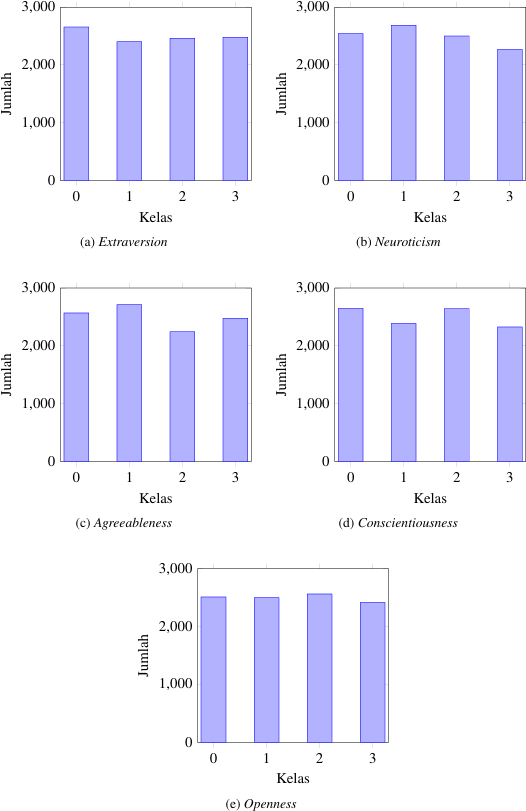
\includegraphics[width=0.62\columnwidth]{figures/fig_label_distribution.png}
  \caption{Class distribution of the five traits after quartile discretisation (x-axis: class; y-axis: number of videos)}
  \label{fig:1}
\end{figure}

Confusion matrices from the first experiments showed that most errors occurred between the two middle classes, whose scores are close to each other and to the centre of a roughly bell-shaped trait distribution. Trait scores are continuous by nature~\cite{radis}, so a boundary between neighbouring middle classes is largely arbitrary. A second label scheme was therefore created by keeping class 0, merging classes 1 and 2 into a single medium class, and relabelling class 3 as class 2. Both schemes are evaluated, and they are reported separately because the three-class task has fewer decision boundaries and is not directly comparable with the four-class task.

\subsection{Frame Selection, Face Cropping, and Auxiliary Features}
Each video is divided into five equal temporal segments, and candidate frames are taken at a stride of five frames within each segment. The quality of candidate frame $j$ is computed as the weighted sum in Equation~(\ref{eq:1}), and the highest-scoring frame of each segment is kept, which gives five frames per video.

\begin{equation}
  Q_j = 0.8\, S_j^{\text{sharp}} + 0.2\, S_j^{\text{align}}
  \label{eq:1}
\end{equation}
Here $S_j^{\text{sharp}}$ is the sharpness score, computed as the variance of the Laplacian of the grayscale frame, and $S_j^{\text{align}}$ is a facial alignment score derived from the MTCNN face landmarks that rewards a centred, symmetric face~\cite{mtcnn}. The weights 0.8 and 0.2 favour sharpness because motion blur is the most common degradation in the clips. When no face is detected in a segment, the first frame of that segment is used, and when fewer than five frames are available the last frame is repeated. Figure~\ref{fig:2} shows an example of the five frames selected for one video.

\begin{figure}[t]
  \centering
  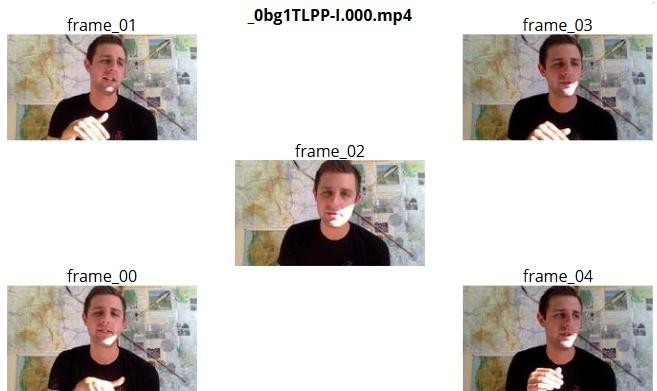
\includegraphics[width=0.92\columnwidth]{figures/fig_best_frames.jpeg}
  \caption{Example of the five best frames selected from one video, one frame per temporal segment}
  \label{fig:2}
\end{figure}

The selected frames are cropped to the MTCNN bounding box and resized to 224 $\times$ 224 pixels, falling back to the whole frame when detection fails. Two auxiliary vectors are then computed for each cropped face. The first is a seven-dimensional emotion probability vector (angry, disgust, fear, happy, sad, surprise, neutral) produced by the DeepFace library~\cite{serengil}, where the complete distribution is used instead of only the dominant label and a neutral-dominant vector replaces failed analyses. The second is an identity embedding extracted with ArcFace~\cite{arcface}, which is used only in the final stage of each label scheme. Pixel values are normalised with ImageNet statistics, and random horizontal flip, rotation, and colour jitter are applied to the training data only.

\subsection{Model Architecture}
The architecture is shown in Figure~\ref{fig:3}. Each of the five frames passes through a Swin Transformer backbone pretrained on ImageNet~\cite{swin} and yields a 512-dimensional facial feature. The five features are aggregated into one video representation. In the baseline configuration, the aggregation is the mean pooling of Equation~(\ref{eq:2}), where $\mathbf{f}_i$ is the feature of frame $i$, $N=5$ is the number of frames, and $\mathbf{F}$ is the video-level feature.

\begin{equation}
  \mathbf{F} = \frac{1}{N}\sum_{i=1}^{N} \mathbf{f}_i
  \label{eq:2}
\end{equation}
\begin{figure}[t]
  \centering
  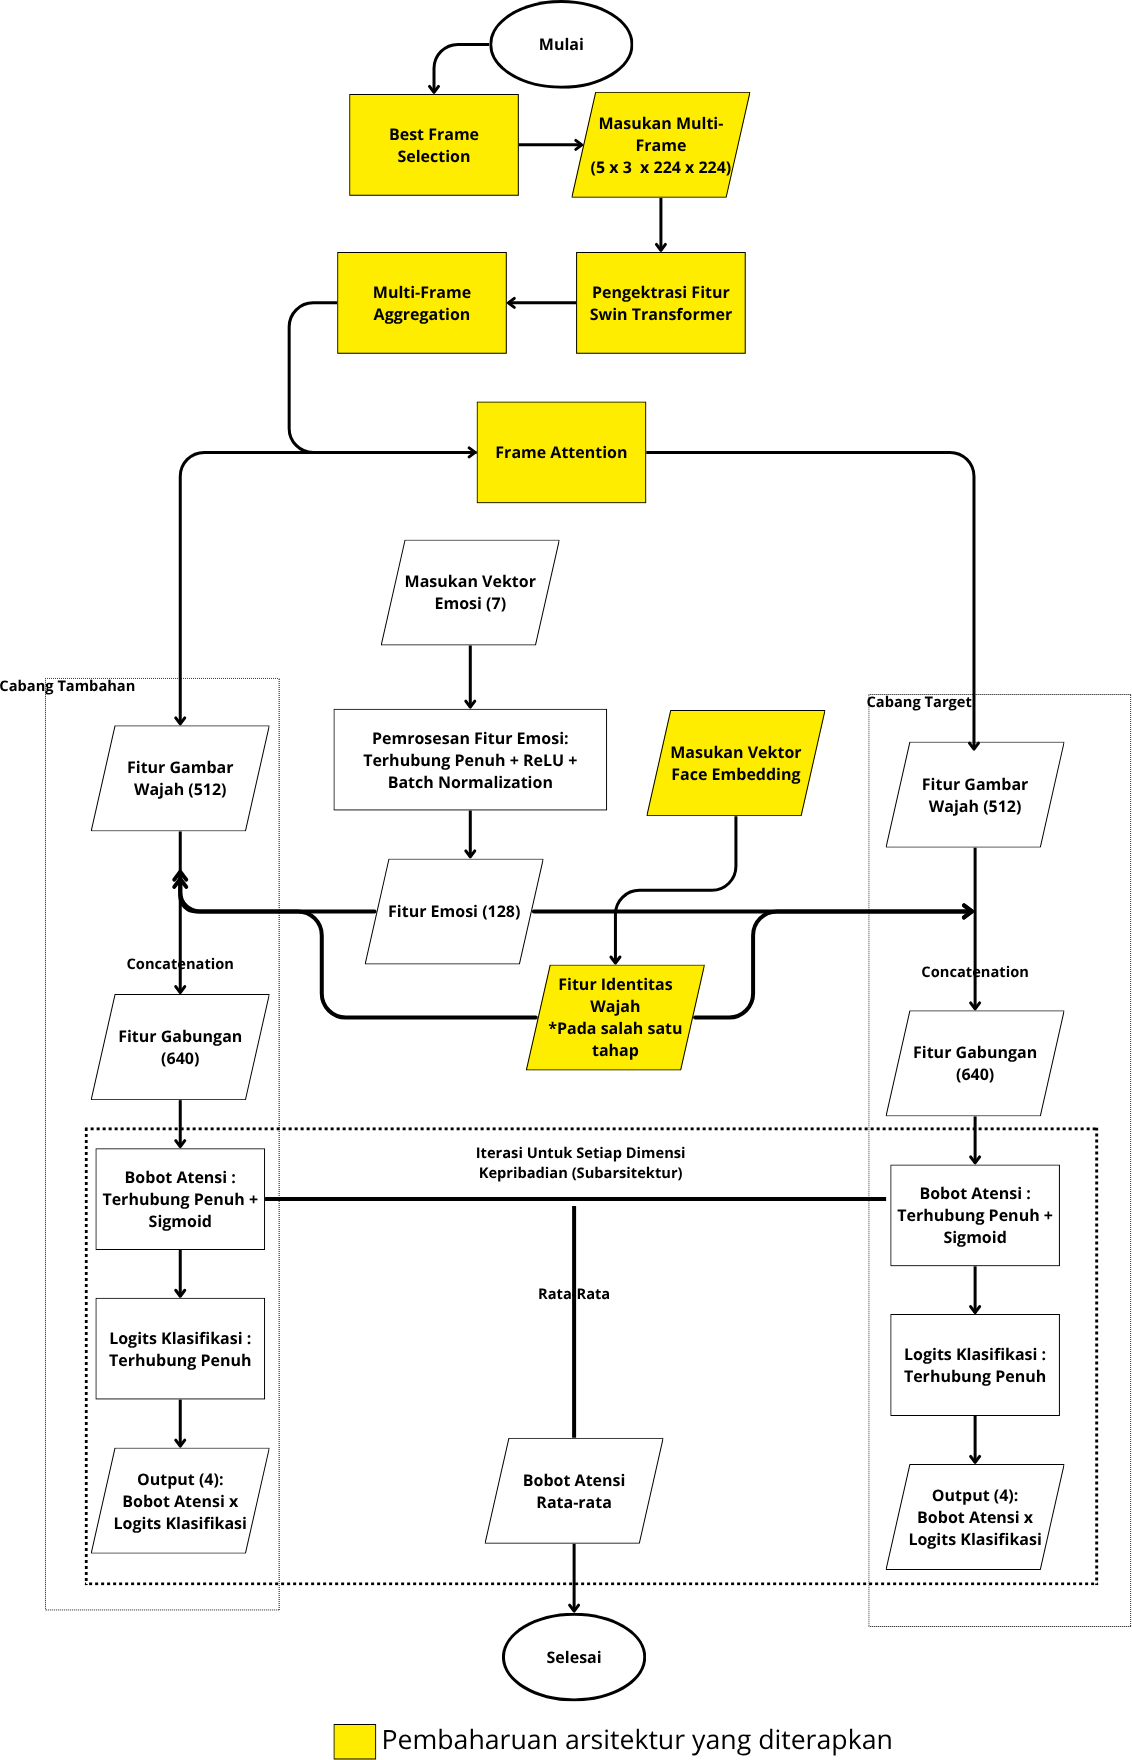
\includegraphics[width=0.85\columnwidth]{figures/fig_architecture.png}
  \caption{Proposed architecture: multi-frame Swin Transformer features are aggregated, fused with emotion and identity features, and classified by the dual-branch Ada-DF head}
  \label{fig:3}
\end{figure}

Frame attention replaces the uniform weights of Equation~(\ref{eq:2}) with learned weights that sum to one, so that informative frames contribute more. Quality-weighted loss scales the training loss of each frame by its quality score, which reduces the influence of blurred or poorly aligned frames during optimisation. The temporal transformer applies self-attention across the five frame features before aggregation so that relations between frames are modelled instead of treating them independently.

The emotion vector passes through a fully connected layer with ReLU and batch normalisation to give a 128-dimensional feature, which is concatenated with the 512-dimensional video feature into a 640-dimensional fused feature, following the emotion integration of the predecessor model~\cite{wardana}. The ArcFace embedding, when used, is concatenated at the same point. The fused feature feeds the two Ada-DF branches~\cite{liu_adadf}. Each branch contains, for every trait, an attention head with a fully connected layer and sigmoid activation, which follows the uncertainty-weighting idea of the Self-Cure Network~\cite{scn}, and a fully connected classifier that outputs the logits of the $C$ classes. The auxiliary branch estimates a label distribution $d^{\text{aux}}$ and, together with a class-level distribution $d^{\text{class}}$, yields the fused target distribution of Equation~(\ref{eq:3}), where $w_{x_i}$ is the attention weight of sample $x_i$.

\begin{equation}
  d^{\text{fused}}_{x_i} = w_{x_i}\, d^{\text{aux}}_{x_i} + \left(1 - w_{x_i}\right) d^{\text{class}}_{x_i}
  \label{eq:3}
\end{equation}
The model is trained with the combined loss of Equation~(\ref{eq:4}), where $L_{\text{kld}}$ is the Kullback--Leibler divergence between the target-branch prediction and $d^{\text{fused}}$, $L_{\text{ce}}$ is the cross-entropy of the auxiliary branch, and $L_{\text{RR}}$ is the rank regularisation loss that separates the attention weights of high-confidence and low-confidence samples. The coefficients $\alpha_1$ and $\alpha_2$ are scheduled with the epoch $\epsilon$ and the threshold epoch $\beta$, with $\alpha_1 = \exp\!\big(-(1-\epsilon/\beta)^2\big)$ and $\alpha_2 = 1$ for $\epsilon \le \beta$, and $\alpha_1 = 1$ and $\alpha_2 = \exp\!\big(-(1-\beta/\epsilon)^2\big)$ otherwise~\cite{liu_adadf}.

\begin{equation}
  L = \alpha_1 L_{\text{kld}} + \alpha_2 L_{\text{ce}} + L_{\text{RR}}
  \label{eq:4}
\end{equation}
\subsection{Experimental Scenarios and Training}
The components were added cumulatively in ten stages, as summarised in Table~\ref{tab:1}. Stages 1 to 5 use the four-class labels. Stages 6 to 10 repeat the same sequence with three classes, except that Stage 6 starts again from the mean-pooling baseline, and each subsequent stage adds one component to the previous one. A single-frame ResNet18 baseline with and without emotion features serves as the reference~\cite{liu_adadf,wardana}.

\begin{table}[t]
  \caption{Experimental stages}
  \label{tab:1}
  \centering
  \footnotesize
  \setlength{\tabcolsep}{3pt}
  \begin{tabular}{ccp{29mm}p{22mm}}
    \toprule
    Stage & Classes & Configuration & Purpose \\
    \midrule
    1 & 4 & Swin + five frames + mean pooling & Baseline \\
    2 & 4 & + frame attention & Frame importance \\
    3 & 4 & + quality-weighted loss & Quality-aware optimisation \\
    4 & 4 & + temporal transformer & Inter-frame relations \\
    5 & 4 & + ArcFace embedding & Identity information \\
    6 & 3 & Stage 1 configuration & Reduced label ambiguity \\
    7 & 3 & + frame attention & Frame importance \\
    8 & 3 & + quality-weighted loss & Quality-aware optimisation \\
    9 & 3 & + temporal transformer & Inter-frame relations \\
    10 & 3 & + ArcFace embedding & Identity information \\
    \bottomrule
  \end{tabular}
\end{table}

All stages used AdamW with an exponential learning-rate scheduler, a maximum of 100 epochs with early stopping after 10 epochs without improvement, and a batch size of 4 with 4 accumulation steps (effective batch size 16) to fit the memory of the GPU. The Ada-DF parameters inherited from the predecessor were fixed, namely $\beta=3$, minimum and maximum weights of 0.2 and 1.0, $\gamma=0.95$, a margin of 0.07, and no label smoothing~\cite{wardana}. Learning rate (searched in $[10^{-5}, 10^{-4}]$), dropout rate ($[0, 0.5]$), and the label-distribution threshold ($[0.5, 0.9]$) were tuned per stage with Optuna~\cite{akiba}, maximising the weighted objective of Equation~(\ref{eq:5}) on the validation data. The selected values are given in Table~\ref{tab:2}. Training was run on a laptop with an NVIDIA GeForce RTX 5060 GPU, supplemented by a remote PC and Google Colab with a Tesla T4 GPU.

\begin{table}[t]
  \caption{Hyperparameters selected by Optuna for each stage}
  \label{tab:2}
  \centering
  \footnotesize
  \setlength{\tabcolsep}{3pt}
  \begin{tabular}{ccccc}
    \toprule
    Stage & Learning rate & Drop rate & Threshold & Best objective \\
    \midrule
    1 & 3.66e-5 & 0.239 & 0.647 & 0.4415 \\
    2 & 4.28e-5 & 0.147 & 0.690 & 0.4438 \\
    3 & 3.49e-5 & 0.189 & 0.687 & 0.4465 \\
    4 & 3.24e-5 & 0.228 & 0.663 & 0.4433 \\
    5 & 2.08e-5 & 0.188 & 0.619 & 0.4462 \\
    6 & 5.09e-5 & 0.217 & 0.786 & 0.5872 \\
    7 & 2.99e-5 & 0.212 & 0.725 & 0.5903 \\
    8 & 3.86e-5 & 0.298 & 0.621 & 0.5887 \\
    9 & 3.91e-5 & 0.253 & 0.892 & 0.5930 \\
    10 & 6.70e-5 & 0.499 & 0.647 & 0.5860 \\
    \bottomrule
  \end{tabular}
\end{table}

\subsection{Evaluation Metrics}
Each trait is evaluated separately with Top-1 accuracy~\cite{touvron} and with precision, recall, and F1-score computed in the one-versus-all manner for multi-class classification~\cite{sokolova}. Because a single network predicts all five traits at once in a multi-output setting~\cite{alzhrani}, the metrics are averaged over the five traits to obtain model-level values. Model selection uses the overall score of Equation~(\ref{eq:5}), where $\overline{F1}$ and $\overline{\text{Acc}}$ are the means of the per-trait F1-score and Top-1 accuracy. The larger weight on F1 reflects the ambiguity and slight imbalance of the classes, and the score also drives early stopping and checkpoint selection.

\begin{equation}
  \text{Overall} = 0.7\,\overline{F1} + 0.3\,\overline{\text{Acc}}
  \label{eq:5}
\end{equation}
Confusion matrices of the best checkpoint of every stage are computed on the 2,000 test videos to analyse where errors occur. The precision, recall, and F1-score reported below are weighted averages over classes, which is why recall equals Top-1 accuracy.

\section{Results and Discussions}
\subsection{Four-Class Results}
Table~\ref{tab:3} summarises the mean test performance of all ten stages. With four classes, the Swin Transformer baseline with mean pooling reached 0.4329 accuracy and 0.4359 F1-score. Adding frame attention raised these values to 0.4376 and 0.4410, and adding quality-weighted loss gave the best accuracy of 0.4458 with an F1-score of 0.4433. The temporal transformer then lowered performance slightly to 0.4374 and 0.4406, and the ArcFace embedding recovered it to 0.4414 and 0.4444, which is the highest four-class F1-score but a lower overall score than Stage 3 (0.4435 against 0.4441).

\begin{table}[t]
  \caption{Mean test performance of each stage (weighted averages over the five traits)}
  \label{tab:3}
  \centering
  \footnotesize
  \setlength{\tabcolsep}{2pt}
  \begin{tabular}{ccC{12mm}C{12mm}C{12mm}C{12mm}}
    \toprule
    Stage & Classes & Top-1 accuracy & Precision & Recall & F1-score \\
    \midrule
    1 & 4 & 0.4329 & 0.4449 & 0.4329 & 0.4359 \\
    2 & 4 & 0.4376 & 0.4501 & 0.4376 & 0.4410 \\
    3 & 4 & 0.4458 & 0.4478 & 0.4458 & 0.4433 \\
    4 & 4 & 0.4374 & 0.4485 & 0.4374 & 0.4406 \\
    5 & 4 & 0.4414 & 0.4530 & 0.4414 & 0.4444 \\
    6 & 3 & 0.5842 & 0.5837 & 0.5842 & 0.5815 \\
    7 & 3 & 0.5999 & 0.6013 & 0.5999 & 0.5907 \\
    8 & 3 & 0.5954 & 0.5964 & 0.5954 & 0.5840 \\
    9 & 3 & 0.5873 & 0.5852 & 0.5873 & 0.5814 \\
    10 & 3 & 0.5913 & 0.5897 & 0.5913 & 0.5853 \\
    \bottomrule
  \end{tabular}
\end{table}

Two observations follow. First, the spread across the five four-class stages is only about 0.013 in accuracy, which is of the same order as the binomial standard error of an accuracy near 0.44 on 2,000 samples (about 0.011), so the ranking of individual components should be read as a tendency instead of a firm ordering. Second, quality-weighted loss produced the largest single accuracy gain (+0.008 over Stage 2), although its F1 gain (+0.002) is smaller than that of frame attention (+0.005). A plausible explanation is that it acts directly on the input quality problem that motivated multi-frame selection, down-weighting blurred or poorly aligned frames, whereas the temporal transformer operates on five frames that were picked from separate segments and therefore do not form a continuous motion sequence. Facial personality cues are also largely static, so modelling temporal dynamics adds parameters without much new information.

The ArcFace embedding was designed to separate identities, not to encode expression or perceived impression. Its small gain is consistent with this mismatch, and it suggests that identity information is only weakly related to the trait labels. The confusion matrices of the four-class stages show that the extreme classes are recognised better than the middle ones. For example, at Stage 3 the recall of Openness is about 0.60 and 0.57 for classes 0 and 3 but only about 0.29 and 0.41 for classes 1 and 2, and the errors are concentrated between neighbouring middle classes.

\subsection{Three-Class Results}
Merging the two middle classes increased the mean accuracy from the 0.43--0.45 range to 0.58--0.60 and the F1-score to 0.58--0.59, with the best configuration at Stage 7 (0.5999 accuracy and 0.5907 F1-score). Beyond Stage 7, additional components did not help: quality-weighted loss, the temporal transformer, and ArcFace gave 0.5954, 0.5873, and 0.5913 accuracy, respectively. The differences between stages again stay within about 0.01--0.02, which is of the order of the sampling error.

The jump of roughly 0.15 in accuracy therefore comes mostly from the label scheme and not from the architecture, and part of it is an artefact of the easier task. With three classes, a chance-level classifier would score 0.33 instead of 0.25, and because the merged middle class holds about half of the test videos (1,007 to 1,062 of 2,000 per trait at Stage 6), always predicting the middle class would already give an accuracy of about 0.50--0.53. The reported 0.58--0.60 is thus a moderate improvement over that majority baseline. The confusion matrices confirm that the model over-predicts the middle class. At Stage 7, the recall of the middle class is about 0.75 for both Conscientiousness and Agreeableness, whereas the recall of the low and high classes is only 0.43--0.49. Reformulating the labels reduces the confusion between neighbouring classes, but it does not give the model the ability to separate low and high levels reliably.

\subsection{Per-Trait Analysis}
Table~\ref{tab:4} gives the per-trait results of the best model of each label scheme. Extraversion is the lowest trait in both schemes, with an accuracy of 0.3880 and an F1-score of 0.3728 at four classes and 0.5540 and 0.5404 at three classes. Agreeableness, Openness, and Conscientiousness are consistently higher, and Neuroticism lies in between.

\begin{table}[t]
  \caption{Per-trait test results of the best four-class model (Stage 3) and the best three-class model (Stage 7)}
  \label{tab:4}
  \centering
  \footnotesize
  \setlength{\tabcolsep}{2pt}
  \begin{tabular}{lC{12mm}C{12mm}C{12mm}C{12mm}}
    \toprule
    Trait & 4-class accuracy & 4-class F1 & 3-class accuracy & 3-class F1 \\
    \midrule
    Openness & 0.4660 & 0.4631 & 0.6105 & 0.6047 \\
    Conscientiousness & 0.4595 & 0.4599 & 0.6140 & 0.6048 \\
    Extraversion & 0.3880 & 0.3728 & 0.5540 & 0.5404 \\
    Agreeableness & 0.4690 & 0.4728 & 0.6105 & 0.6018 \\
    Neuroticism & 0.4465 & 0.4477 & 0.6105 & 0.6019 \\
    Mean & 0.4458 & 0.4433 & 0.5999 & 0.5907 \\
    \bottomrule
  \end{tabular}
\end{table}

This ordering agrees with the view that Agreeableness and Openness have comparatively consistent facial correlates, such as open or friendly expressions, while Extraversion is expressed mainly through social behaviour, energy, and communication style that a short frontal clip and a facial crop capture only partly. Note that this interpretation is not tested in this study, because no experiment isolates behavioural cues. Conscientiousness and Neuroticism show intermediate performance, which may reflect cues such as tension or calmness that appear in some frames but not consistently.

\subsection{Comparison with Previous Work}
Table~\ref{tab:5} compares the best models with the original Ada-DF baseline~\cite{liu_adadf} and its emotion-augmented extension~\cite{wardana} under the final test run. With four classes, the model with emotion features and quality-weighted loss improves the mean accuracy and F1-score of the emotion-augmented predecessor from 0.4058 and 0.3863 to 0.4441 and 0.4422, i.e., by 3.8 and 5.6 points. Relative to the original Ada-DF, the gains are 4.5 and 8.1 points. The final comparison run reports slightly different figures from the per-stage evaluation in Table~\ref{tab:3} for the same configuration (for example 0.4441 instead of 0.4458 accuracy at Stage 3), so the two sets of numbers should not be mixed.

\begin{table*}[t]
  \caption{Mean test performance compared with previous work}
  \label{tab:5}
  \centering
  \footnotesize
  \setlength{\tabcolsep}{4pt}
  \begin{tabular}{p{62mm}ccccc}
    \toprule
    Model & Classes & Top-1 accuracy & Precision & Recall & F1-score \\
    \midrule
    Ada-DF~\cite{liu_adadf} & 4 & 0.3995 & 0.3666 & 0.3985 & 0.3610 \\
    Ada-DF + emotion~\cite{wardana} & 4 & 0.4058 & 0.3870 & 0.4040 & 0.3863 \\
    Ada-DF + emotion + quality-weighted loss (ours) & 4 & 0.4441 & 0.4460 & 0.4441 & 0.4422 \\
    Ada-DF + emotion + frame attention (ours) & 3 & 0.5841 & 0.5885 & 0.5841 & 0.5680 \\
    \bottomrule
  \end{tabular}
\end{table*}

The three-class model reaches 0.5841 accuracy and 0.5680 F1-score, which is about 17.8 and 18.2 points above the emotion-augmented predecessor. This difference should not be read as an architectural gain, because the predecessor was not evaluated with three classes, and the task is easier for the reasons given in Section~3.2. The fair comparison with the earlier models is the four-class one, where the improvement is smaller but real. The overall pattern also points to a broader lesson: once a modern backbone and multi-frame input are in place, further architectural components contribute marginally, while the label representation determines most of the attainable performance.

\subsection{Limitations and Future Work}
Several limitations should be kept in mind. Each configuration was trained once, and no confidence intervals or multiple seeds are reported, so differences of 0.01--0.02 between stages are not statistically established. Only one dataset with perceived-personality annotations from crowd workers was used, and these annotations reflect the impressions of raters instead of self-reported traits, which limits what the predictions can be said to measure. The three-class results are affected by the majority-class effect discussed above, and the tuned hyperparameters differ per stage, which confounds the comparison between components to some extent. Finally, predicting personality from faces raises validity and fairness concerns, and the model should not be used for consequential decisions such as hiring without independent validation.

Future work should replace discrete classes with continuous, ordinal, or soft-label representations so that the arbitrary middle boundaries are avoided, since the experiments indicate that label design is the main bottleneck. Backbones pretrained for expression or impression recognition instead of identity could provide more suitable features, and complementary modalities such as speech and text are likely to help traits like Extraversion that are weakly visible in the face. Larger and more diverse datasets with more objective annotation would reduce the rater bias, and tuning each configuration under a shared budget would give a cleaner comparison of the components.

\section{Conclusions}
This study extended the Ada-DF framework for Big Five personality prediction from facial video by replacing the ResNet18 backbone with a Swin Transformer, by using five quality-selected frames per video, and by combining emotion probabilities and ArcFace identity embeddings with frame attention, quality-weighted loss, and a temporal transformer. Selecting frames by sharpness and facial alignment and aggregating them produced stable representations, and with four equal-frequency classes the best configuration reached a mean Top-1 accuracy of 0.4441 and an F1-score of 0.4422 on the 2,000 test videos, improving on the emotion-augmented Ada-DF baseline (0.4058 and 0.3863) and on the original Ada-DF (0.3995 and 0.3610). Among the components, quality-weighted loss gave the largest accuracy gain, whereas the temporal transformer and ArcFace embeddings produced no meaningful gain, probably because the selected frames are not a continuous sequence and identity embeddings carry little trait-related information. Merging the two middle classes increased the mean accuracy to 0.58--0.60 and the F1-score to about 0.58--0.59, but this increase mainly reflects a simpler classification problem, and the merged middle class sets a majority baseline of about 0.50--0.53, which the model exceeds only moderately. Across both label schemes Agreeableness, Openness, and Conscientiousness were predicted better than Neuroticism and, in particular, Extraversion, which suggests that facial appearance carries weaker information about socially expressed traits. The results indicate that, once a modern backbone and multi-frame input are used, the main bottleneck of facial personality prediction lies in the representation of the labels and the characteristics of the data rather than in further architectural complexity. Subsequent research should therefore examine continuous or ordinal targets, report results over repeated runs, and test whether additional modalities can capture the behavioural aspects of personality that the face does not convey.


% ---------------------------------------------------------------------
%  ACKNOWLEDGEMENTS (max three lines; no supervisors)
% ---------------------------------------------------------------------
\section*{Acknowledgements}
The authors declare no conflict of interest. This research received no specific
grant from any funding agency in the public, commercial, or not-for-profit
sectors. % TODO: authors to confirm

% ---------------------------------------------------------------------
%  REFERENCES (IEEE style, 8 pt, minimum 25 with DOI)
% ---------------------------------------------------------------------
{\footnotesize
\bibliographystyle{IEEEtran}
\bibliography{references}
}

\end{document}
